\documentclass[11pt]{amsart}
\usepackage[marginratio=1:1, headheight=27pt,
footskip = 13pt, a4paper, total={6.5in, 8in}]{geometry}                % See geometry.pdf to learn the layout options. There are lots.
\geometry{letterpaper}                   % ... or a4paper or a5paper or ...
%\geometry{landscape}                % Activate for for rotated page geometry
%\usepackage[parfill]{parskip}    % Activate to begin paragraphs with an empty line rather than an indent
\usepackage{graphicx}
\usepackage[font=small,labelfont=bf]{caption} % Required for specifying captions to tables
\usepackage{dirtytalk}
%\usepackage[version=3]{mhchem}
%\usepackage{subcaption}
\usepackage{subfig}
%\usepackage{epstopdf}
\usepackage{booktabs}
\usepackage[compact,small]{titlesec}
\usepackage{complexity}
%\usepackage[sc, osf]{mathpazo} % add possibly `sc` and `osf` options
%\usepackage{eulervm}
%\usepackage{textcomp}

\clubpenalty = 10000
\widowpenalty = 10000
%\usepackage[altbullet]{lucidabr}
\usepackage{float}
\usepackage{siunitx}
\usepackage[justification=centering]{caption}
\usepackage[
colorlinks = true,
urlcolor = blue
]{hyperref}
\usepackage{mathrsfs}
\usepackage{amssymb}
\usepackage{mathtools}
\usepackage{amsmath}
\usepackage{amsthm}
\renewcommand\qedsymbol{$\blacksquare$}

\usepackage[section]{placeins}
\DeclareGraphicsRule{.tif}{png}{.png}{`convert #1 `dirname #1`/`basename #1 .tif`.png}

%\usepackage[swedish]{babel}
\usepackage[T1]{fontenc}
\usepackage[utf8]{inputenc}

\usepackage{comment}
\usepackage{enumitem}
\titleformat{\section}[block]{\large\scshape\centering}{\thesection.}{1em}{}
\titleformat{\subsection}[block]{\large}{\thesubsection.}{1em}{}

\usepackage{pgfplots}
\pgfplotsset{compat = 1.15}

\usepackage{listings}
\lstset{basicstyle=\ttfamily,breaklines=true}
\usepackage{color} %red, green, blue, yellow, cyan, magenta, black, white
\definecolor{mygreen}{RGB}{28,172,0} % color values Red, Green, Blue
\definecolor{mylilas}{RGB}{170,55,241}

%\usepackage{times}
%\usepackage{kpfonts}
%\usepackage{txfonts}
%\usepackage{newtx}
%\usepackage{stix}
%\usepackage[osf,proportional]{libertine}
%\usepackage{lmodern}
\usepackage[charter]{mathdesign}

\usepackage{microtype}
%\usepackage{stix}
\usepackage[compact,small]{titlesec}
\titleformat*{\section}{\large\bfseries\sffamily}

\titleformat*{\subsection}{\small\bfseries\sffamily}
\titleformat*{\subsubsection}{\small\bfseries\sffamily}
%\renewcommand{\section}{\section*}
\newcommand{\ibits}{\{0, 1\}^*}
%\renewcommand{\familydefault}{\sfdefault}
\usepackage{marginnote}
\renewcommand*{\marginfont}{\color{red}\sffamily\footnotesize}
\usepackage{hyperref, xcolor}

%\usepackage{makeidx}
\definecolor{winered}{rgb}{0.5,0,0}
\hypersetup{
     pdfauthor={JAG},
     pdfsubject={Hyperlinks in LaTeX},
     pdftitle={main.tex},
     pdfkeywords={LaTeX, PDF, hyperlinks}
%    colorlinks=false,
     pdfborder={0 0 0},
%You can set individual colors for links as below:
colorlinks=true,
  linkcolor=winered,
urlcolor={winered},
filecolor={winered},
citecolor={winered},
allcolors={winered}
}

\usepackage[english]{babel} 
\usepackage[
backend=biber,
style=numeric,
hyperref=true,
%natbib
]{biblatex}
\DeclareLanguageMapping{swedish}{swedish-apa}
\addbibresource{Komplexitetsteori.bib}

\usepackage[T1]{fontenc}
\usepackage{tikz-cd}
%\usepackage{fouriernc}

\usepackage{thmtools}
\usepackage{fancyhdr}

\usepackage{csquotes}

\usepackage{polynom}
\polyset{%
   style=C,
   delims={\big(}{\big)},
   div=:
}

\newsavebox{\myheadbox}
\fancypagestyle{normalpage}
{
%\begin{flushright}
\lhead{
Jonas Conneryd
}
%\end{flushright}
\rhead{\url{conneryd@kth.se}}
\chead{MM8042 Algebraic Topology}
\cfoot{\thepage}
}
\fancyhf{}
\fancypagestyle{firstpage}
{
%\begin{flushright}
\lhead{
Jonas Conneryd \\ \url{conneryd@kth.se}}
%\end{flushright}
\rhead{970731-7559  \\
\the\year
}
\chead{\Large{\scshape{\textbf{Homework 5} \\ \vspace{-4pt}\normalsize\textbf{ MM8042 Algebraic Topology}}}}
\cfoot{\thepage}
}

\pagestyle{normalpage}


\declaretheoremstyle[headfont=\bfseries\scshape]{normalhead}
\interfootnotelinepenalty=10000
%\title{\vspace{-2cm}\textbf{\textsf{ Homework 3}}}
\date{}
%\author{Jonas Conneryd \\
%conneryd@kth.se \\ 970731-7559}

\renewcommand{\C}{\mathbb{C}}
\newcommand{\GL}{\mathsf{GL}}
\newcommand{\Z}{\mathbb{Z}}
\renewcommand{\R}{\mathbb{R}}
\newcommand{\Res}{\mathsf{Res}^{D_{2n}}_{\langle x\rangle}}
\newcommand{\triv}{\mathbb{1}}
\newcommand{\Char}{\mathsf{Char}}
\newcommand{\Fix}{\mathsf{Fix}}
\newcommand{\Span}{\mathsf{Span}}
\newcommand{\Tr}{\mathsf{Tr}}
\newcommand{\Ker}{\mathsf{Ker}}
\renewcommand{\Im}{\mathsf{Im}}
\newcommand{\Cent}{\mathsf{Cent}}
\newcommand{\Id}{\mathsf{Id}}

\begin{document}
%\maketitle
\thispagestyle{firstpage}
\theoremstyle{normalhead}
\newtheorem{problem}{Problem}
\newtheorem{lemma}{Lemma}


\begin{problem}
  For points $y_0, \ldots, y_k$ in a convex set $Z$, let $\overline{y_0 \ldots y_k} = \frac{y_0 + \ldots + y_k}{k+1}$ denote their barycenter.
\begin{enumerate}[font=\scshape,label=\textbf{(\Alph*)}]
  \item Let
  \[
\Delta^n = [y_0, \ldots, y_n] = \left\{t_0 y_0 + \ldots + t_n y_n | t_i \geq 0, \sum_i t_i = 1\right\}
  \]
  be the $n$-dimensional simplex with our usual notation. Let $(i_0, \ldots, i_n)$ be a permutation of $(0, \ldots, n)$. Prove that
  \[
[\overline{y_{i_0}}, \overline{y_{i_0}y_{i_1}}, \ldots , \overline{y_{i_0}\ldots y_{i_n}}] =\{t_0 y_0 + \ldots + t_n y_n | t_{i_0} \geq t_{i_1} \geq \ldots t_{i_n} \}.
  \]

  \item Prove that the simplices $[\overline{y_{i_0}}, \overline{y_{i_0}y_{i_1}}, \ldots , \overline{y_{i_0}\ldots y_{i_n}}]$, ranging over all permutations $(i_0, \ldots, i_n)$ of $[n] = (0, \ldots, n)$, triangulate $\Delta^n$ (that is, their union is $\Delta^n$ and the intersection of any two is a face of both).
\end{enumerate}

\end{problem}
\begin{proof}[Solution]
  \hfill

\begin{enumerate}[font=\scshape,label=\textbf{(\Alph*)}, wide]
  \item By definition, we have
  \[
  \begin{aligned}
[\overline{y_{i_0}}, \overline{y_{i_0}y_{i_1}}, \ldots , \overline{y_{i_0}\ldots y_{i_n}}] &= \left\{t_0 y_{i_0} + t_1 \frac{y_{i_0} + y_{i_1} }{2} + \ldots t_n\frac{\sum_{i=0}^n t_i}{n+1}\right\} \\
&=\left\{y_{i_0}\sum_{i = 0}^n\frac{t_i}{i+1} + y_{i_1} \sum_{i = 1}^n\frac{t_i}{i+1} +y_{i_2} \sum_{i = 2}^n\frac{t_i}{i+1} + \ldots + y_{i_n}\frac{t_n}{n+1}\right\} \\
&=\left\{y_{i_0}\sum_{i = 0}^n\frac{t_i}{i+1} + y_{i_1}\left( \sum_{i = 0}^n\frac{t_i}{i+1} -t_0 \right) + \ldots + y_{i_n}\left( \sum_{i = 0}^n\frac{t_i}{i+1} - \sum_{i = 0}^{n-1}\frac{t_i}{i+1} \right)\right\} \\
&= \left\{s_{i_0} y_{i_0} + s_{i_1} y_{i_1} + \ldots + s_{i_n} y_{i_n}\right\}
\end{aligned}
\]
Since $t_i \geq 0$ for all $i$, we get by the above that $s_{i_0} \geq s_{i_1} \geq \ldots \geq s_{i_n}$. Since the terms in all the sums have strictly increasing denominators and the sum of the $t_i$ is 1, the maximal value for each $s_{i_k}$ is its value when the first $t_i$ appearing in the corresponding sum (see the second row in the above equation) is set to 1 and all other $t_k$ to 0. Therefore all $s_{i_k}$ are bounded by 1, with the bound being sharp for $s_{i_0}$. By convexity of $Z$, the set described in this paragraph is a subset of $\Delta^n$. Finally, the sum $\sum_k s_{i_k}$ is 1 since
\[
\begin{aligned}
\sum_{k= 0}^n s_{i_k} &= \sum_{i = 0}^n\frac{t_i}{i+1} + \left( \sum_{i = 0}^n\frac{t_i}{i+1} -t_0 \right) + \ldots + \left( \sum_{i = 0}^n\frac{t_i}{i+1} - \sum_{i = 0}^{n-2}\frac{t_i}{i+1} \right) + \left( \sum_{i = 0}^n\frac{t_i}{i+1} - \sum_{i = 0}^{n-1}\frac{t_i}{i+1} \right) \\
&= (n+1)\frac{t_n}{n+1} + n\frac{t_{n-1}}{n} + \ldots + 2 \frac{t_1}{2} +  t_0 \\
&= \sum_{i=0}^n t_i,
\end{aligned}
\]
which by definition is 1. In summary,
$[\overline{y_{i_0}}, \overline{y_{i_0}y_{i_1}}, \ldots , \overline{y_{i_0}\ldots y_{i_n}}] =\{s_0 y_0 + \ldots + s_n y_n | s_{i_0} \geq s_{i_1} \geq \ldots \geq s_{i_n} \}$, which was the sought result.

\item Let $i$ be a permutation. Let $[\overline{y_{i_0}}, \overline{y_{i_0}y_{i_1}}, \ldots , \overline{y_{i_0}\ldots y_{i_n}}] = \left\{t_0 y_{i_0} + t_1 \frac{y_{i_0} + y_{i_1} }{2} + \ldots t_n\frac{\sum_{i=0}^n t_i}{n+1}\right\} = \{s_0 y_0 + \ldots + s_n y_n | s_{i_0} \geq s_{i_1} \geq \ldots s_{i_n} \} \coloneqq A_i$.
A face of $A_i$ obeys the same conditions as above, with the added constraint that one or more of the $t_i$ are zero. How does this look in terms of the $s_i$? As in \textbf{(A)}, we have
\[
\left\{t_0 y_{i_0} + t_1 \frac{y_{i_0} + y_{i_1} }{2} + \ldots t_n\frac{\sum_{i=0}^n t_i}{n+1}\right\} = \left\{y_{i_0}\sum_{i = 0}^n\frac{t_i}{i+1} + y_{i_1} \sum_{i = 1}^n\frac{t_i}{i+1} +y_{i_2} \sum_{i = 2}^n\frac{t_i}{i+1} + \ldots + y_{i_n}\frac{t_n}{n+1}\right\}.
\]
From this point of view, we see that setting $t_i = 0$ gives equality between $s_i$ and $s_{i+1}$. Hence, we can identify faces of $A_i$ with equalities in the sequence of relations $s_{i_0} \geq \ldots \geq s_{i_n}$.

Let $i, k$ be permutations and consider the intersection $A_{ik} = A_i\cap A_k$. By \textbf{(A)}, we can think of this set as
\[
A_{ik} = \{s_0 y_0 + \ldots + s_n y_n | s_{i_0} \geq s_{i_1} \geq \ldots s_{i_n} \text{ and }  s_{k_0} \geq s_{k_1} \geq \ldots s_{k_n}\}.
\]
We consider the restriction on $A_{ik}$ more closely:
\[
\begin{aligned}
s_{i_0} &\geq s_{i_i} \geq \ldots \geq s_{i_r} \geq \ldots \geq s_{i_n} \\
s_{k_0} &\geq s_{k_i} \geq \ldots \geq s_{k_r} \geq \ldots \geq s_{i_n}.
\end{aligned}
\]
 Suppose $i_l = k_l$ for $l = 0,\ldots, r$, and $i_{l+1} \neq l_{l+1}$. Then $k_{l+1}$ is $i_s$ for some $s>r$ since all the lower indices fulfil $i_l = k_l$, (and therefore $s_{k_{r+1}}$ is to the right of $s_{i_{r+1}}$ in the above picture. Therefore we have the relation $s_{i_{r+1}} \geq s_{k_{r+1}}$. At the same time, by a symmetric argument $s_{k_{r+1}} \geq s_{i{r+1}}$, so we get equality for all $s_{i_j}$ with indices $j$ between $r+1$ and $s$ (which is guaranteed to be at least two elements). We can repeat this process for higher indices, which leads to constraints on $A_ik$ which will be of the form $s_{i_0} R_0 s_{i_1} R_{1} \ldots R_{n-1} s_{i_n}$, where the $R_l$ are either $\geq$ or $=$. By the above discussion, this defines a face of $A_i$, since at least one $R_l$ will be $=$ for two distinct permutations $i, k$ as we saw above. Entirely symmetrically, this process leads to constraints on $A_{ik}$ of the form $s_{k_0} R'_0 s_{k_1} R'_{1} \ldots R'_{n-1} s_{k_n}$, which by the above discussion defines a face of $A_k$. Hence the intersection of $A_i$ and $A_k$ is a face of both of them.


Next, we show that the union of all $A_i$ is $\Delta^n$. By \textbf{(A)} we have
\[
\begin{aligned}
\bigcup_{\text{permutations } i}  [\overline{y_{i_0}}, \overline{y_{i_0}y_{i_1}}, \ldots , \overline{y_{i_0}\ldots y_{i_n}}] = \bigcup_{\text{permutations } i} \{t_0 y_0 + \ldots + t_n y_n | t_{i_0} \geq t_{i_1} \geq \ldots t_{i_n} \} \\
= \{t_0 y_0 + \ldots + t_n y_n | t_{i_0} \geq t_{i_1} \geq \ldots t_{i_n} \text{ or } t_{i'_0} \geq t_{i'_1} \geq \ldots t_{i'_n} \text{ or } \ldots\},
\end{aligned}
\]
that is, $\bigcup_i A_i$ is the set of all sums$ \sum_k t_ky_k$ where $t_k \geq 0, \sum_k t_k = 1$ and the $t_k$ are ordered according to \emph{some} linear ordering out of the set of all linear orderings of $[n]$ (which is in one-to-one correspondence with the set of all permutations on $n+1$ indices). Since any configuration of the $t_i$ will obey some linear ordering out of the set of all linear orderings, we get that $\sum_i A_i$ is just the set of all sums $\sum_k t_ky_k$ where $ t_k \geq 0,\forall k$ and $\sum_k t_k =1$. This is precisely $\Delta^n$.

In conclusion, the simplices $[\overline{y_{i_0}}, \overline{y_{i_0}y_{i_1}}, \ldots , \overline{y_{i_0}\ldots y_{i_n}}]$, ranging over all permutations of $[n]$, triangulate $\Delta^n$. The proof is complete.
\end{enumerate}
\end{proof}
\newpage

\begin{problem}

  Let $X$ be the space obtained from the closed unit disk $D^2$ by first deleting the interiors of two disjoint subdisks in the interior of $D^2$ and then identifying the three resulting boundary circles together via homeomorphisms preserving clockwise orientations of these circles.

  Describe a CW structure on $X$, and use it to calculate the cellular (and therefore also the singluar) homology of $X$.
\end{problem}
\begin{proof}[Solution]
We equip $X$ with the following CW-structure, consisting of one 2-cell, three 1-cells and one 0-cell:
\begin{center}
  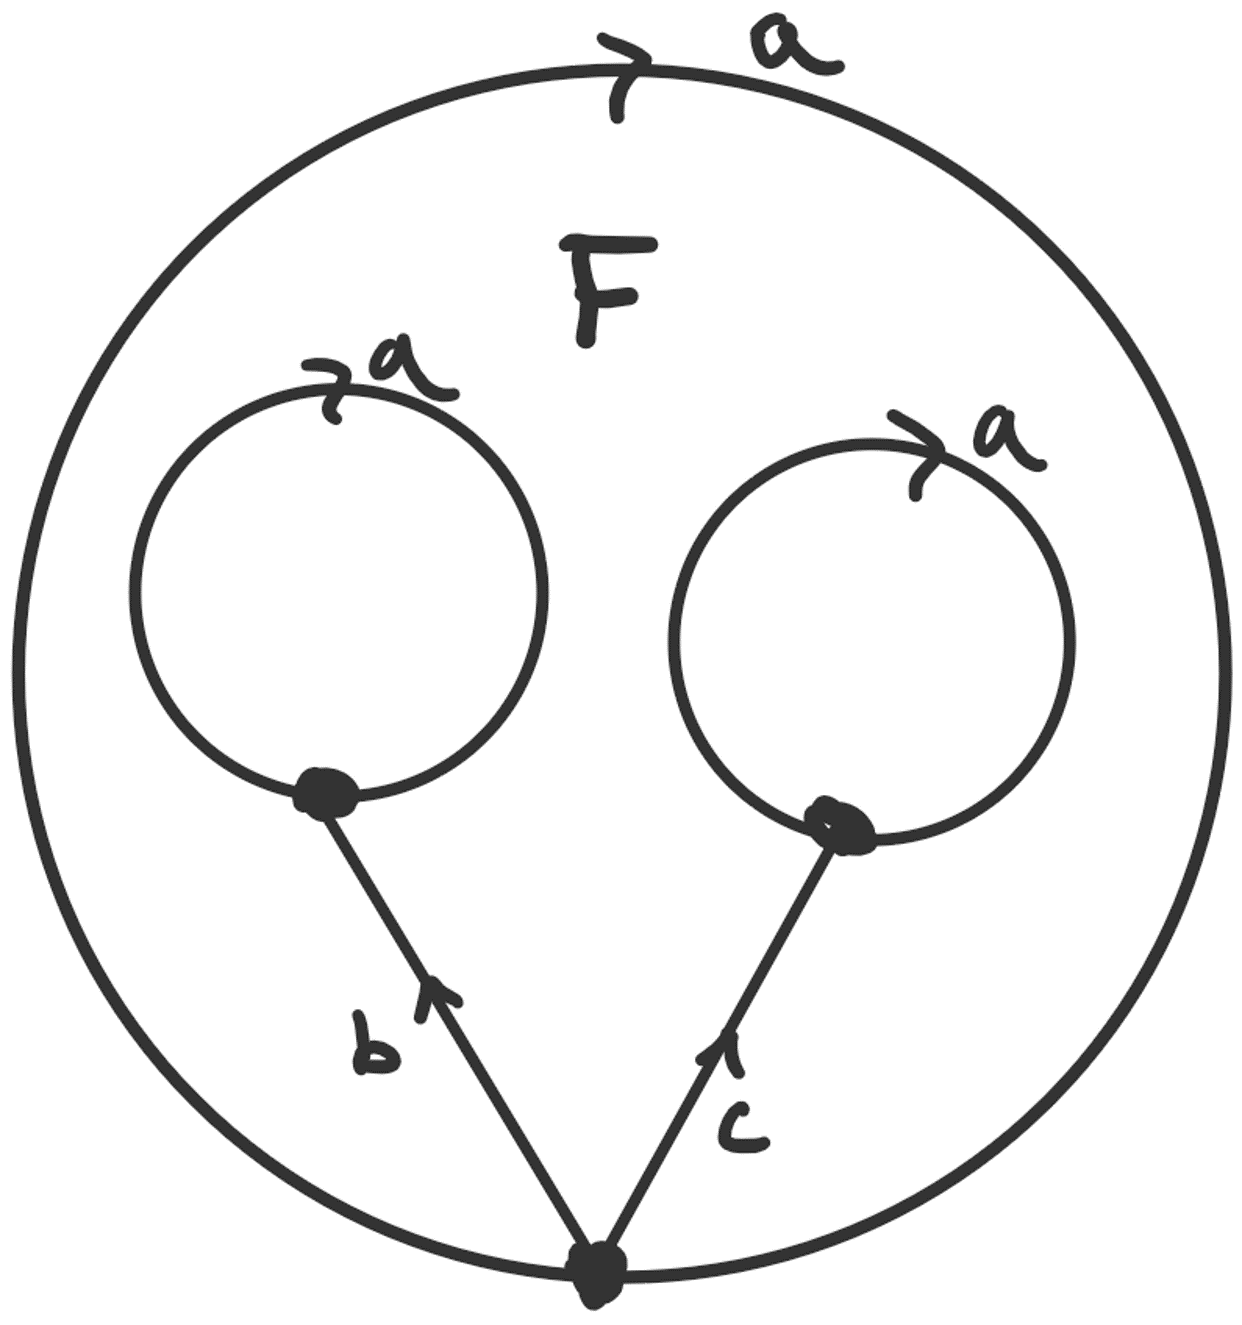
\includegraphics[width = 0.3\linewidth]{CW.png}
\end{center}
Starting at the bottom vertex, a bit to the right of $a$, we can follow along the 1-cells to see that the attaching map for the 2-cell amounts to attaching along the word $aca^{-1}c^{-1}ba^{-1}b^{-1}$. Since the sum of the exponents of $a$ in the word is $-1$ and the sum of the exponents of $b$ and $c$ in the word is 0, we can use the Cellular Boundary Formula to deduce that $d_2(F) = -a$. Furthermore, since $X$ is connected and there is only one 0.cell (all points are identified with each other in our CW structure), we know that $d_{1}$ is the zero map. Moreover $d_0$ is the zero map. All maps $d_n$ for $n\geq 3$ are also the zero maps since all homology groups $H_n(X)$ are zero for $n\geq 3$, which follows from the fact that the highest dimensional $n$-skeleton is $X^2$ in $X$. We have a sequence
\[
\begin{tikzcd}
  0 \arrow[r, "d_3"] & H_2(X^2, X^1) \arrow[r, "d_2"] & H_1(X^1, X^0) \arrow[r, "d_1"] & H_0(X^0, X^{-1}) \arrow[r, "d_0"] & 0
\end{tikzcd}
\]
which is
\[
\begin{tikzcd}
  0 \arrow[r, "d_3"] & \Z \arrow[r, "d_2"] & \Z^{\oplus 3} \arrow[r, "d_1"] & \Z \arrow[r, "d_0"] & 0.
\end{tikzcd}
\]
$H_1(X^1, X^0)$ is generated by $a, b, c$. We have
\[
\begin{aligned}
H_2(X) &= \Ker(d_2)/\Im(d_3) = 0; \\
H_1(X) &= \Ker(d_1)/\Im(d_2) = \langle a, b, c \rangle/\langle -a \rangle \cong \Z^{\oplus2}; \\
H_0(X) &= \Ker(d_0)/\Im(d_1) \cong \Z.
\end{aligned}
\]
\end{proof}


\end{document}
